\documentclass[aps,pre,12pt,preprint,%
	onecolumn,showpacs,showkeys,nofootinbib]{revtex4-1}
%Chinese
	\usepackage[UTF8,fontset=fandol]{ctex}
	\xeCJKsetup{underdot = {
		boxdepth=0pt, format=\huge, depth=.4em
	}}
%	\usepackage[datesep=/]{datetime2} % Use default
	\DeclareTextFontCommand{\textbf}{\sffamily}
%Presenting
	\usepackage[table]{xcolor}
	\usepackage{graphicx}
	\usepackage[space]{grffile}
	\usepackage[font=small,format=plain,%
		labelfont=bf,textfont=it,%
		singlelinecheck=false]{caption}
	\usepackage[above]{placeins}
%	\usepackage{float} % Cause trouble for table footnotes
	\usepackage{wrapfig}
	\usepackage{tabularx,array,booktabs,multirow,bigstrut}
	\newcolumntype{C}[1]{>{\hsize=#1\hsize%
		\centering\arraybackslash}X}
	\newcommand{\minitab}[2][l]{%
		\begin{tabular}{#1}#2\end{tabular}}
	\usepackage{setspace,dcolumn}
	\usepackage{subfig}
	\usepackage{psfrag,epsfig}
%MathSetting
	\let\latexointop\ointop
	\usepackage{amsmath,bm,amssymb,esint,extarrows}
	\usepackage{upgreek,textcomp,mathrsfs}
	\usepackage[only,sslash]{stmaryrd}
	\usepackage{nicefrac,eqnarray}
%	\usepackage{amsthm} % Enable when necessary
%	\usepackage[mathscr]{eucal} % Enable when necessary
	\usepackage{mathtools,physics,siunitx}
	\usepackage{stackengine,varwidth}
	\usepackage{tikz}
	\usepackage{resizegather,empheq}
	\usetagform{default}
	\usepackage{calligra,fourier-orns}
	% Keep \oint unchanged by esint
	\let\ointop\undefined
	\let\ointop\latexointop
	% Define a scriptr 
	\DeclareMathAlphabet{\mathcalligra}{T1}{calligra}{m}{n}
	\DeclareFontShape{T1}{calligra}{m}{n}{<->s*[2.2]callig15}{}
	\newcommand{\scriptr}{\mathcalligra{r}\,}
	\newcommand{\rvector}{\pmb{\mathcalligra{r}}\,}
	% Useful shorthand
	\DeclarePairedDelimiter\ave{\langle}{\rangle}
	\newcommand\inlineeqno{\stepcounter{equation}\ (\theequation)}
	\newcommand{\sinc}{\operatorname{sinc}}
	\newcommand{\mbb}[1]{\mathbb{#1}}
	\newcommand{\mrm}[1]{\mathrm{#1}}
	\newcommand{\mcal}[1]{\mathcal{#1}}
	\newcommand{\tup}[1]{\textup{#1}}
	% Scaling and positioning
	\newcommand\scalemath[2]{\scalebox{#1}{\mbox{\ensuremath{\displaystyle #2}}}}
	\newcommand\raisemath[2]{\raisebox{#1\depth}{${#2}$}}
	\empheqset{box=\nicebox}
	% Presenting
	\newcommand*\nicebox[1]{\fbox{\hspace{1em}\addstackgap[5pt]{#1}\hspace{1em}}}
	\sisetup{%
		redefine-symbols=false,%
		separate-uncertainty=true,%
		range-phrase=\,\textasciitilde\,,%
		arc-separator = \,}
	\allowdisplaybreaks[2]
%ParagraphSetting
	\setlength{\parskip}{.3\baselineskip}
	\usepackage[defaultlines=2,all]{nowidow}
	\postdisplaypenalty=50
%PageSetting
	\usepackage{titlesec}
	\titleformat*{\section}{\large\bfseries}
	\usepackage[colorlinks=true,linkcolor=blue]{hyperref}
	\newcommand{\texstringonly}[1]{%
		\texorpdfstring{#1}{}}
	\usepackage[vmargin={3.5cm,4cm},hmargin=3cm,%
		footnotesep=\baselineskip]{geometry}
%	\usepackage[bottom]{footmisc} % Cause trouble for table footnotes
	\usepackage{changepage}
	% Autoref names
	\renewcommand{\tableautorefname}{\tablename}
	\renewcommand{\figureautorefname}{\figurename}
	% List settings
	\usepackage{enumitem}
	\setlist{itemsep=0pt,topsep=0pt,labelindent=\parindent,leftmargin=0pt,itemindent=*}
	% Some redefined lengths
	\setlength{\headsep}{1.6\baselineskip}
%	\setlength{\footnotesep}{3\parskip} % Use when necessary
	% Header
	\usepackage{fancyhdr,lastpage}
	\pagestyle{fancy}
%	\fancyhf{} % Clear default settings; disabled for now
	\cfoot{--\ \thepage\,/\,\pageref{LastPage} \ --}
	\setlength{\footskip}{2\baselineskip}
	\renewcommand{\headrulewidth}{0.1pt}
	\renewcommand{\headrule}{
		\ifnum\value{page}=1\relax\else
			\vbox to 2pt{
			\hbox to \headwidth{\dotfill}\vss}
		\fi}
	\fancypagestyle{titlepagestyle}{%
		\fancyhead{}
		\chead{
			\vspace{2.5\baselineskip}
			
\includegraphics[width=.75\linewidth]{../PKUPhy}}
	}
	% Separator
	\newcommand{\newparagraph}{\pagebreak[3]\noindent%
		\hfil
		~\raisebox{-4pt}[10pt][10pt]{\decofourright~~~~~~~~\decofourleft}~ %
		\par
	}
%	% Background % Use when necessary
%	\usepackage{background} %Waterstamp package
%	\SetBgContents{...的实验报告} %Waterstamp to prevent copying
%	\SetBgScale{5} %Waterstamp setting
	% Essay format
	\renewcommand\appendixname{附录}
	\renewcommand\abstractname{}%摘要
	\renewcommand\tablename{表}
	\renewcommand\figurename{图}
	\renewcommand\refname{参考文献}
	\makeatletter
	\def\@pacs@name{\songti\zihao{-4}{\bf PACS码:}}
	\def\@keys@name{\songti\zihao{-4}{\bf 关键词:}}
	\def\Dated@name{日期:}
	\def\Received@name{\zihao{-5}{接收} }
	\def\Revised@name{\zihao{-5}{修订} }
	\def\Accepted@name{\zihao{-5}{采纳} }
	\def\Published@name{\zihao{-5}{发表} }
	\makeatother
	\linespread{1.5}
	\renewcommand{\labelenumi}{\alph{enumi}.}
	\leftmargini=20mm
	\newcommand{\supercite}[1]{\textsuperscript{\,%
		[\citenum{#1}]}}
	\let\fancycite\cite
	\renewcommand{\cite}[1]{\textup{\fancycite{#1}}}
	% Math line spacing
	\newlength{\djot}
	\setlength{\djot}{\jot}
	\newcommand{\restorejot}{\setlength{\jot}{\djot}}

%Miscellaneous
%	\newcommand{\tabindent}{\hspace{2em}}
%FourierTransform
	\newcommand{\fourierf}{\mathscr F}
\begin{document}
%Basic Data
	\title{%
	\texstringonly{\hfil\\[2\baselineskip]}
	\sf\LARGE%
		扫描电镜的构造、使用\\
		及聚光镜电流对像质影响的探究%
	\texstringonly{\vspace{3ex}}}
	\author{\fangsong\large%
		Bryan%
	\vspace{2mm}}
	\affiliation{\it%
		北京大学物理学院~~学号:\normalfont 1500000000\,}
	\date{\today}
	\keywords{扫描电子显微镜(SEM)\ 电子透镜\ 聚光镜电流\ %
		像质\ 分辨率}
	\email{guesswhat@email.addr;}

\begin{abstract}
\vspace{10mm}
\begin{spacing}{1.5}\normalsize
\setlength{\parskip}{.3\baselineskip}
%	200—300字,
%	说明用什么方法做了什么事,
%	由此得到什么结果和结论,
%	有何意义.
%	不用缩略词,不用第一人称.
%%%%%%%%%%%%%%%%%%%%%%%%%%%%%%%%
	扫描电子显微镜是研究物质微观形貌及组分的重要实验装置。本实验回顾了扫描电镜的基本结构、工作原理及调节办法,在此基础上探究了驱动电子透镜中的聚光镜电流对成像质量的影响。
	
	具体而言,本实验考察了 \numrange{400}{650} 范围内、间隔步长50的6个聚光镜电流值对应的 \SI{1}{k} 和 \SI{10}{k} 倍放大图像,用直观及半定量(频谱分析)的办法比较了图像的像质。结果表明,随电流增大,图像分辨率增大;且在聚光镜电流较大的情况下,噪声对像质有所影响。这一结果与初步的理论分析基本吻合。
\end{spacing}
\end{abstract}

\maketitle
\thispagestyle{titlepagestyle}

%	\item 课程实验报告应假定读者既不是已知全部实验细节的指导教师,也不是缺少专业知识的公众,而是同领域的实验研究者,或审稿人. 不能要求读者要在读过课程讲义后才能读懂课程实验报告.
%	\item 公式、图和表要分别用阿拉伯数字编列序号. 公式和图表要达到可发表的质量.
%	\item 凡不是自己独立思考得到的内容都应该引参考文献. 不能大段引用同一参考文献. 对复杂问题,应该优先考虑引用参考文献得到结果. 对简单一些的问题才鼓励独立思考.
%	\item 较长的推导和说明可以作为附件提交,不占用报告篇幅.
%	\item 思考题不是报告的组成部分. 应另起一页附在报告的最后.
\section{引言}
%%	研究论文引言一般包含以下内容:
%%	(1)所研究领域背景和现状;
%%	(2)有待研究的问题;
%%	(3)本研究的目的、主要内容和结果;
%%	(4)结果的意义.\par
%%	在写实验报告的引言时,同学可以假想自己是第一个做类似研究的人.\par
%%	引言一定要切合报告正文,不能漫无目的地介绍背景. 要快速地将读者引导到报告主题上,并作较深入的讨论.\par
%%	引言篇幅可以在较大范围内变化,但最长不应超过报告文字篇幅的1/3.\par
%%	引言撰写可以参考实验讲义,可以复述,但不能复制讲义上的任何一句话.\par
%%%%%%%%%%%%%%%%%%%%%%%%%%%%%%%
	\vspace{-2ex}
	1900年前后,最好的光学显微镜分辨率已接近其理论极限$\sim\SI{200}{\nm}$, 这一限制源于光的衍射行为及可见光的波长下限。为了制造更高分辨率的显微镜以看清更小层次的物质,人们不得不从新的思路出发突破该瓶颈。
	
	\setlength{\jot}{0pt}
	1924年前后,为了解决旧量子论中难以调和的诸多困难,德布罗意(Louis de Broglie)在其发表的博士论文 \cite{de1924recherches} 中提出了一种全新的量子化思路;德布罗意由爱因斯坦的光量子假定出发,推而广之,认为实物粒子同样具有波粒二象性,其\textit{相波}(phase wave)波长为:
	\begin{equation}
		\lambda = \frac{h}{p}
	\end{equation}
	该关系式与光量子的动量公式$p = \frac{h}{\lambda}$完全一致。对于电子而言,在非相对论情形下,$p = \sqrt{2mE} = \sqrt{2meU}$, 其中$U$为加速电压,则有:
	\begin{equation}
		\lambda \approxeq \sqrt{\frac{\SI{150}{\V}}{U}}\,\si{\angstrom}
		\label{eq:deBroglieLambda}
	\end{equation}
	
	相波的假定确认了实物粒子可类比电磁波进行研究,即电子束的运动可与光束的传播类比;且据 \eqref{eq:deBroglieLambda}, 高能电子的相波波长可以显著小于可见光波长,这启示我们可以实物粒子为媒介进行显微探测,从而突破可见光的分辨极限。
	
	物质的波动性随后便得到了实验证实\footnote{%
		例如,参见\cite{thomson1927diffraction}. 
	},并由薛定谔(E. Schrödinger)、波恩(M. Born)等人在理论上严格化。在此基础上,类比光学显微镜,考虑电子\CJKunderdot{透射},人们设计了\textit{透射电子显微镜}(TEM\footnote{%
		TEM是transmission electron microscopy的缩写。
	}),这于1932年前后首次实现,随后不久便获得了高于光学显微镜的分辨率\supercite{ruska1980early};利用电子在表面上的“反射”(严谨而言,是偏角充分大的各类散射),进一步设计了\textit{扫描电子显微镜}(scanning electron microscope, SEM)。
	
\newpage
	SEM利用\textit{电子光学}原理,以电子束代替光束对样品表面进行扫描,收集散射电子及X射线等辐射信号、样品电流信号并加以分析,从而获得样品表面结构、分析样品基本成分。
	
	在SEM的发明过程中,德国物理学家Max Knoll做出了重要的探索性的工作(\textit{参见\cite{knoll1935aufladepotentiel}});在此基础上,与现代原理基本一致的扫描电子显微镜于随后的1937年由德国物理学家Manfred von Ardenne发明\supercite{mcmullan1995scanning}。如今,性能最好的 SEM 分辨率已达到 \SI{.4}{\nm} 以下\supercite{Nanotech86:online}。
	
	相比传统的光学显微镜,SEM 的信号来源要丰富的多,因而有着更加强大的功能。如今SEM已成为化学、生物、材料等许多领域中的重要显微、分析技术。
	
	本实验关注SEM最为基本的信号与功能,即利用散射产生的二次电子(secondary electron, SE)进行样品形貌分析;选取了二次电子成像的一项关键参数,即电子聚光镜电流,探究其对成像的影响,从一较小的角度具体展现SEM的基本性能及其决定因素。\vspace{-6ex}
\section{理论}
	\vspace{-2ex}
	虽说电镜、光学显微镜的类比基础依赖于物质的波动性,但初步的计算分析可利用经典电磁学的方法实现;这实际上是\textit{几何光学极限}的后果,由此分析外场对电子束的作用规律即为(几何)电子光学。具体而言,类比:外加静电磁场$\sim$透镜,起聚光等作用;静电场$\sim$介质,使光线(电子束)发生偏折。此结论基于下述电磁学事实:
	\begin{itemize}[noitemsep]
	\item 带电粒子在等电势区内沿直线运动;
	\item 穿过不同电位区的界面时运动方向改变。
	\end{itemize}
	相应地,磁场$\sim$各向异性介质,详见\cite{textbook}. 
	
	定量分析,电子的运动方程可写为作用量形式:
	\begin{equation}
		\var\int_\mcal{L} \mu\dd{s} = 0
	\end{equation}
	其中$\mu$为广义动量沿轨迹$\mcal{L}$的切向分量;此式与几何光学中的费马原理一致。
\pagebreak
	
	在非相对论极限下,作为例子,进一步考虑纯静电势$\phi$,略去比例系数,有\supercite{textbook}:
	\begin{equation}
		\mu \simeq \phi^{1/2}
	\end{equation}
	$\mu$即电子光学折射率;与光学折射率$n$相比,$\mu$可变范围广、在空间中连续分布,但分布形式受麦克斯韦方程的约束,不可任取。
	
	在旋转对称、傍轴近似下,电子轨迹方程的解完全类似与几何光学光线。由此构造扫描电镜的电子光学系统,示意图如 \ref{fig:semScheme} 所示。
	
	\begin{figure}[!h]
	\vspace{.8ex}
	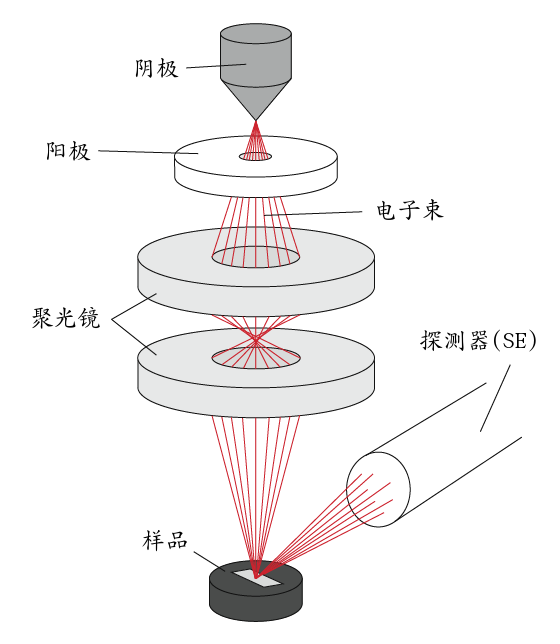
\includegraphics[width=.6\linewidth]{SEMscheme.png}
	\caption[电子光学示意图]{电子光学系统示意图\footnote{%
		据公共资源修改得到:
		\url{https://www.eng-atoms.msm.cam.ac.uk/RoyalSocDemos/SEM}
	}}\vspace{1ex}
	\raggedright\small
	\textit{\hphantom{说明}%
		此为电子光路的原理示意图。聚光镜为电磁透镜,其相对强度由聚光镜电流$i$控制;实际装置中还有若干光学器件(光阑、矫正镜、物镜等)及额外的探测装置(如\tup{X}射线探测器等),这些装置在此原理图中未有体现。
	\vspace{1ex}}
	\label{fig:semScheme}
	\end{figure}
	
	电子束入射样品产生的信号种类及本实验关注的信号——二次电子的主要形成机制如图 \ref{fig:outputSignal}, \ref{fig:SEmech} 所示。
	\begin{figure}[!h]
	\vspace{-3.5ex}
	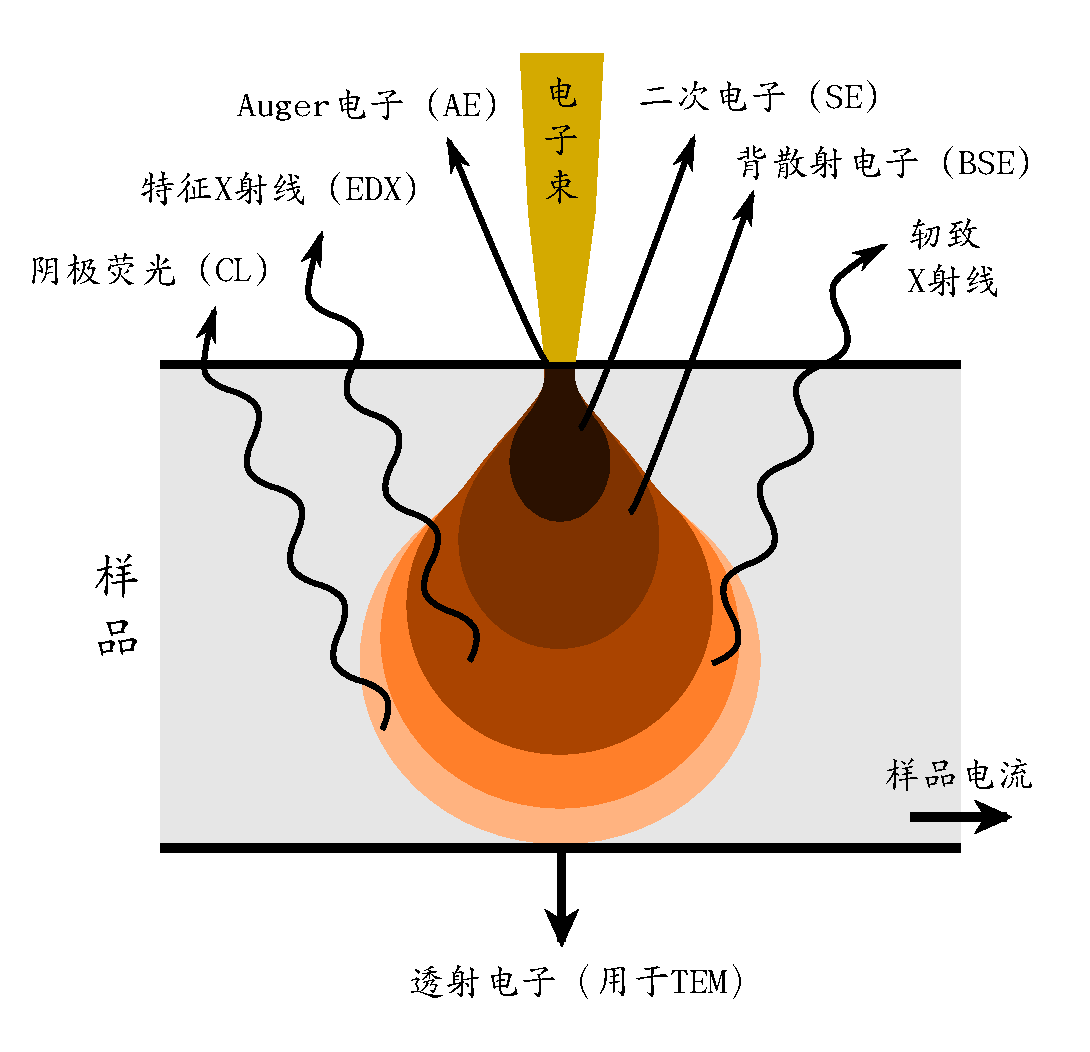
\includegraphics[width=.72\linewidth]{outputSignal.pdf}\vspace{-1.5ex}
	\caption[输出信号]{电子束正入射样品产生的信号种类及其对应层次\footnote{%
		据开源资源修改得到:
		\url{https://en.wikipedia.org/wiki/File:Electron_Interaction_with_Matter.svg}
	},参见\cite{textbook}. }\vspace{1ex}
	\raggedright\small
	\textit{\hphantom{说明}%
		由图可见,二次电子主要源于样品表面附近(若干纳米的薄层,且于入射电子束横向不远处),可以较为忠实地体现样品的表面形貌,即利用二次电子信号重构的样品形貌图像可以具有较高的分辨率。
	\vspace{1ex}}
	\label{fig:outputSignal}
	\end{figure}\FloatBarrier
	
	综上可见,扫描电镜二次电子成像的大致过程为,首先利用电子光学系统使电子束汇聚为充分细的“探针”,偏转电子束方向使电子探针在样品表面扫描,收集对应点逸出的二次电子,进一步分析得到样品表面的形貌。
	
	由此可见,探针的尺度与成像质量密切相关。在其他条件最优化的前提下,探针尺度越纤细,像的分辨程度越高。
	
	\begin{figure}[!h]
	\vspace{-3ex}
	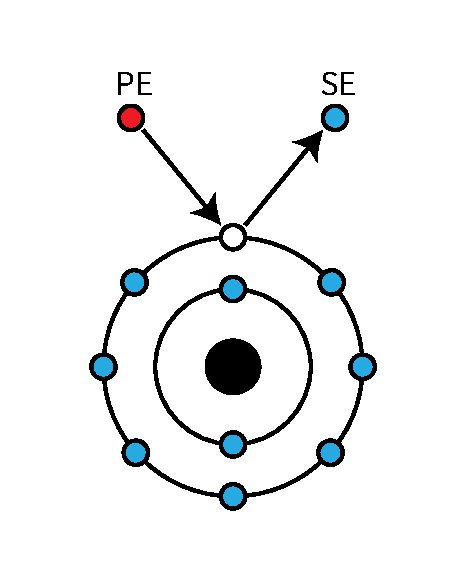
\includegraphics[width=.35\linewidth]{SEmech.pdf}\vspace{-2ex}
	\caption[二次电子机制]{二次电子的主要形成机制\footnote{%
		据开源资源修改得到:
		\url{https://en.wikipedia.org/wiki/File:Electron_emission_mechanisms.svg}
	},参见\cite{textbook}. }\vspace{1ex}
	\raggedright\small
	\textit{\hphantom{说明}%
		实验中习惯上将能量低于 \SI{50}{\eV} 的信号电子统称为二次电子,它主要由逸出的价电子或弱束缚的导带电子构成,如上所示;其中,\tup{PE} (primary electron) 为入射电子。
	\vspace{1ex}}
	\label{fig:SEmech}
	\end{figure}
\section{实验装置}
%%	在此部分需要将实验条件交待清楚到别人能重复你的实验结果的程度. 此外,还需表明你已尽了最大努力来提高实验精度和结果的可靠性. 简单的不确定度估计可以在此节给出,复杂一些的可以放到分析讨论部分.\par
%%	实验条件不仅是指直接影响实验结果的实验参量,而且还包括影响实验质量和可靠性的因素,如室温、空气湿度、基真空、原材料纯度等.\par
%%	作为教学实验报告,此节写详细一点没有坏处.\par
%%	成段有叙述,必要才分节。
%%%%%%%%%%%%%%%%%%%%%%%%%%%%%%%
	本实验采用北京中科科仪生产的SEM, 型号为KYKY-EM3200. 包含二次电子探测装置和X射线探测装置;其分辨本领为 \SI{60}{\angstrom} 即 \SI{6}{\nm}, 放大倍数:15\,\textasciitilde\,\SI{20}{k}. 仪器的工作真空度为 \SI{2.66e-3}{\Pa}, 实验中通过机械泵--分子泵级联抽取获得。
	
	实际操作中,真空度由真空计及手控盒上的VAC示数给出。本实验中,抽真空至VAC示数200(最大)、真空计示数$\SI{7.5e-6}{Torr} < \SI{9.0e-6}{Torr} \sim \SI{1.2e-3}{\Pa}$时,认为达到工作要求。后续操作基本上在计算机(PC)软件上进行
	
	首先,加 \SI{30}{\kV} 高压、设定初始聚光镜电流$i = 550$, 对比度$\sim 60$, 放大倍数小于100, 此时荧幕上可见噪点;在此基础上,通过手控盒上的FILAMENT旋钮加灯丝电流,逐步加至6左右。最终手控盒显示发射电流EMI在 \numrange{80}{100} 区间内,PC上图像亮度近极大值。此时仪器的初始调整基本完成,可以开始显微成像了。
	
\newpage
	本实验中观察的样品为MgF\textsubscript{2}晶体;观察区域的选定可通过样品台外部的旋钮实现,提供5个调节自由度:X, Y, Z, 台面俯仰及绕轴心轴的转动。
	
	实验中,影响像质的主要可调参数依次为:\textbf{聚光镜电流$i$、电对中、聚焦}(物镜电流、工作距离),以及呈现图像时的\textbf{亮度、对比度}。后续操作中,固定放大倍率 \SI{10}{k} 或 \SI{1}{k}, 选择统一的样品区域,依次调整$i$为400, 450, 500, 550, 600和650, 再逐一调整其余参数使图像最优化,且使各图像的\CJKunderdot{表观}亮度、对比度基本一致,以便于比较;由此探究$i$对像质的影响。
\section{结果与分析}
%	实验结果应尽量以图表的形式给出. 每一个图表都应该是完整的,即阅读图表时可以不必依赖正文.\par
%	依自己意愿,实验结果和对结果的分析讨论既可分为两节也可合在一节.\par
%
%	每个图一般包含:图名、轴名、轴、刻度、标尺、数据点、曲线、图例、标注和图注等部分. 应尽量让读者不看正文就能基本理解图的含意.\par
%	逐点测量得到的函数关系要同时用表格和图给出. 需要作比较的多条曲线要画在同一图上.\par
%	为避免读者在图表和正文间反复跳跃阅读,在正文中也要对图表作必要的说明.\par
%
%	对于预料之外的实验结果,必须首先小心证明其可靠性.读者只有在相信你的实验结果时才愿意花时间看你的分析.\par
%	必须用文字归纳整理出正式的实验结果或结论.可信的实验结果是课程报告最重要的内容.作为一个实验物理工作者,分析解释出错并不丢脸,实验结果不被采信则是致命的.\par
%	教学实验的结论往往是预先知道的. 所以,教师更关心的是你的说理过程. 一般说来,单由课内实验的结果不足以能得到明确的结论. 此时,你可以引用他人的研究结果来帮助帮助自己的论证,但必须注明出处. \par
%	确实不能得到明确结论时,可以给出几种可能结论并指出可以再做哪些实验来帮助作进一步的判断.\par
%	总之,分析讨论部分要做到: 论据要valid,论证要reasonable,结论要convincing.\par
%%%%%%%%%%%%%%%%%%%%%%%%%%%%%%
	实验中获得的电镜像如图 \ref{fig:photoOriginal} 所示;相应地,不同倍率、$i$值下的最优化参数如下表所示。观察表中数据,可见一部分参数的最优化值随$i$有显著变化。
	
	\begin{table}[!h]
	\caption[最佳工作参数]{聚光镜电流$i$对应的最佳工作参数}
	\footnotesize
	\vspace{-2\baselineskip}
	\begin{flushleft}\normalsize
		\hspace{3em}\textbf{%
			\SI{10}{k} 倍}\vspace{-1.5ex}
	\end{flushleft}
	\begin{tabularx}{.85\linewidth}{
		C{.5} C{.8} C{.8}
		C{1} C{.5} C{.8}
	}
	 \toprule\midrule
		$i$ &
		电对中 &
		物镜电流 &
		工作距离 / $\si{\mm}$ &
		亮度 & 对比度 \\
	 \midrule
	  400   & $(-6, 6)$ & 651.48 & 5.0   & $-1.4$  & 40.4 \\
	  450   & $(-6, 6)$ & 649.22 & 5.0   & $-1.6$  & 46.3 \\
	  500   & $(-6, 6)$ & 647.86 & 5.0   & $-1.8$  & 52.5 \\
	  550   & $(-6, 6)$ & 646.58 & 5.0   & $-2.1$  & 57.6 \\
	  600   & $(-6, 6)$ & 645.89 & 5.0   & $-2.3$  & 32.4 \\
	  650   & $(-6, 6)$ & 645.22 & 5.0   & $-2.7$  & 67.1 \\
	 \midrule\bottomrule
	\end{tabularx}
	\begin{flushleft}\normalsize
		\hspace{3em}\textbf{%
			\SI{1}{k} 倍}\vspace{-1.5ex}
	\end{flushleft}
	\footnotesize
	\begin{tabularx}{.85\linewidth}{
		C{.5} C{.8} C{.8}
		C{1} C{.5} C{.8}
	}
	 \toprule\midrule
		$i$ &
		电对中 &
		物镜电流 &
		工作距离 / $\si{\mm}$ &
		亮度 & 对比度 \\
	 \midrule
	    400   & $(-6, 6)$ & 651.69 & 5.0   & $-0.2$  & 40.4 \\
	    450   & $(-6, 6)$ & 650.22 & 5.0   & $-1.0$  & 47.8 \\
	    500   & $(-6, 6)$ & 649.25 & 5.0   & $-1.4$  & 54.1 \\
	    550   & $(-6, 6)$ & 647.38 & 5.0   & $-1.8$  & 60.0 \\
	    600   & $(-6, 6)$ & 647.00 & 5.0   & $-2.1$  & 64.7 \\
	    650   & $(-6, 6)$ & 645.55 & 5.0   & $-2.5$  & 70.2 \\
	 \midrule\bottomrule
	\end{tabularx}
	\label{tab:bestValues}
	\end{table}
\clearpage
\FloatBarrier\thispagestyle{empty}
\newgeometry{margin=.05cm}
	\begin{minipage}{\linewidth}
	\vspace{-3.85\baselineskip}\hspace{-7.5em}
	\begin{minipage}[c]{.6\linewidth}
	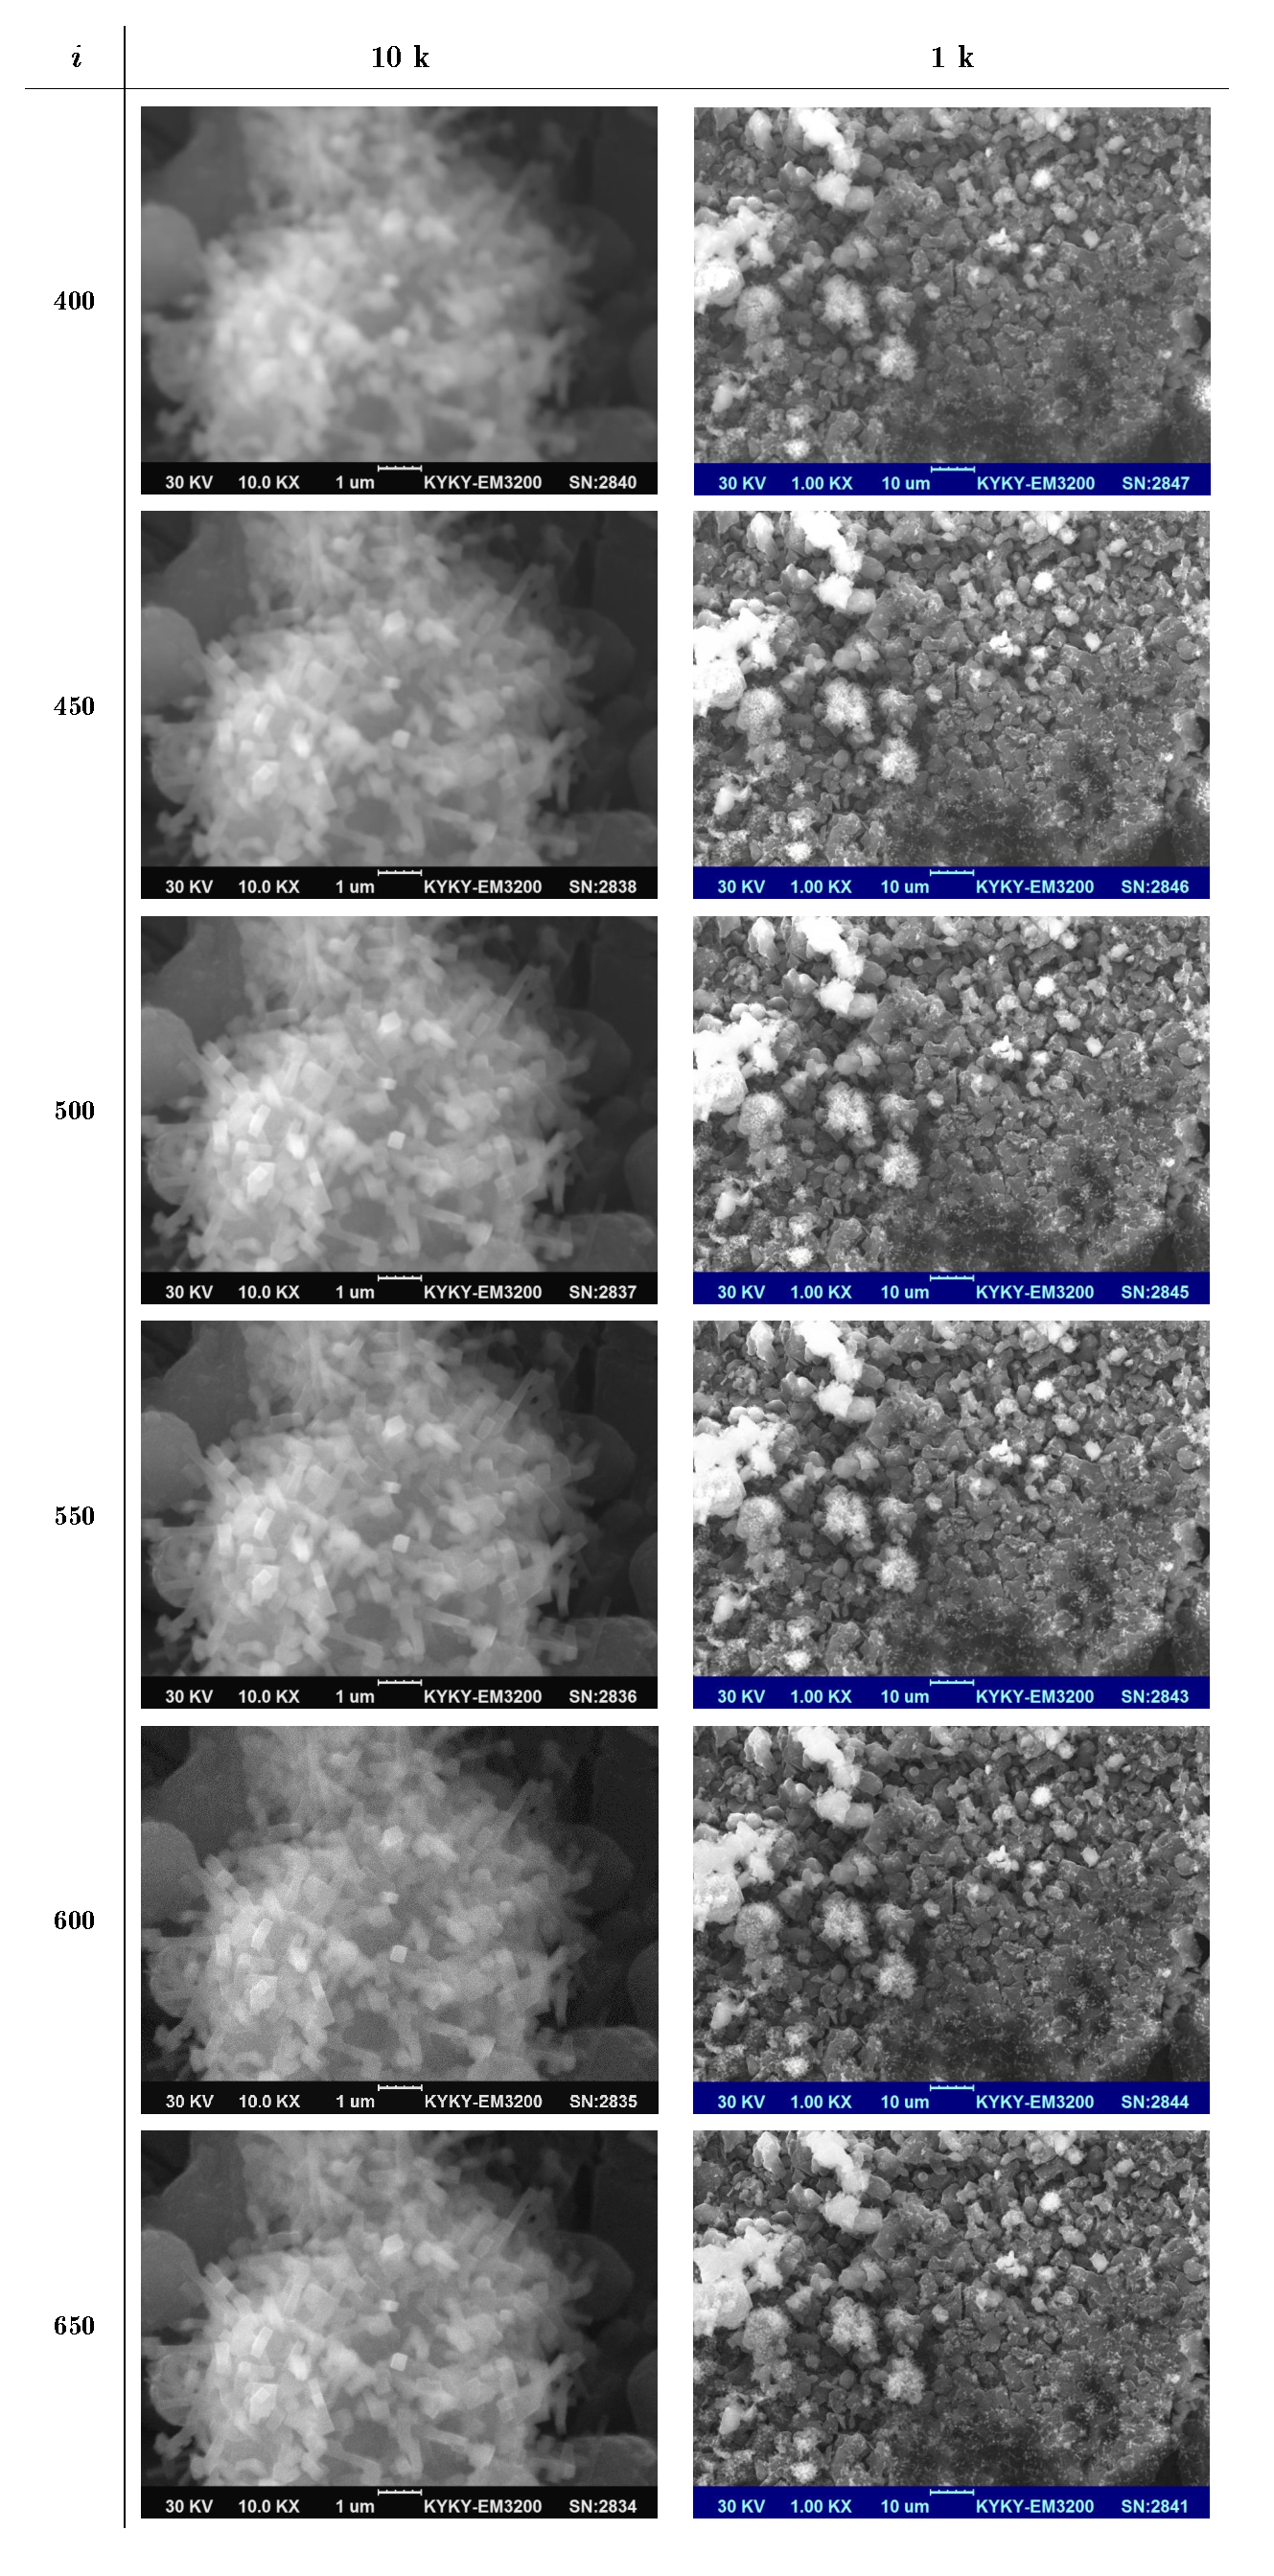
\includegraphics[width=\linewidth]{photoGrid.pdf}
	\end{minipage}
	\begin{minipage}[c]{.3\linewidth}
	\captionof{figure}[电镜图像]{特定$i$值下的最优化%
		扫描电镜像}
	\textit{\hphantom{说明}%
		其中,$i$指代聚光镜电流,图像中的 \tup{10.0 KX}, \tup{1.00 KX} 及标题中的 \SI{10}{k}, \SI{1}{k} 字样代表放大倍数。\tup{30 KV}字样指的是加恒定高压 \SI{30}{\kV}, \tup{SN. }为图片的序列号。
	\vspace{1ex}}\par
	\textit{\hphantom{分析}%
		由图可见,直观上 \SI{10}{k} 倍电镜像的“清晰度”(分辨率)随$i$增大而逐渐增加,在$i = 650$的电镜像中隐约可见“噪点”;而对 \SI{1}{k} 倍电镜像而言,像质差异并不明显。
	\vspace{1ex}}
	\label{fig:photoOriginal}
	\end{minipage}
	\end{minipage}
\restoregeometry
\FloatBarrier

\FloatBarrier\thispagestyle{empty}
\newgeometry{margin=.05cm}
	\begin{minipage}{\linewidth}
	\vspace{-3\baselineskip}\hspace{-6em}
	\begin{minipage}[c]{.625\linewidth}
	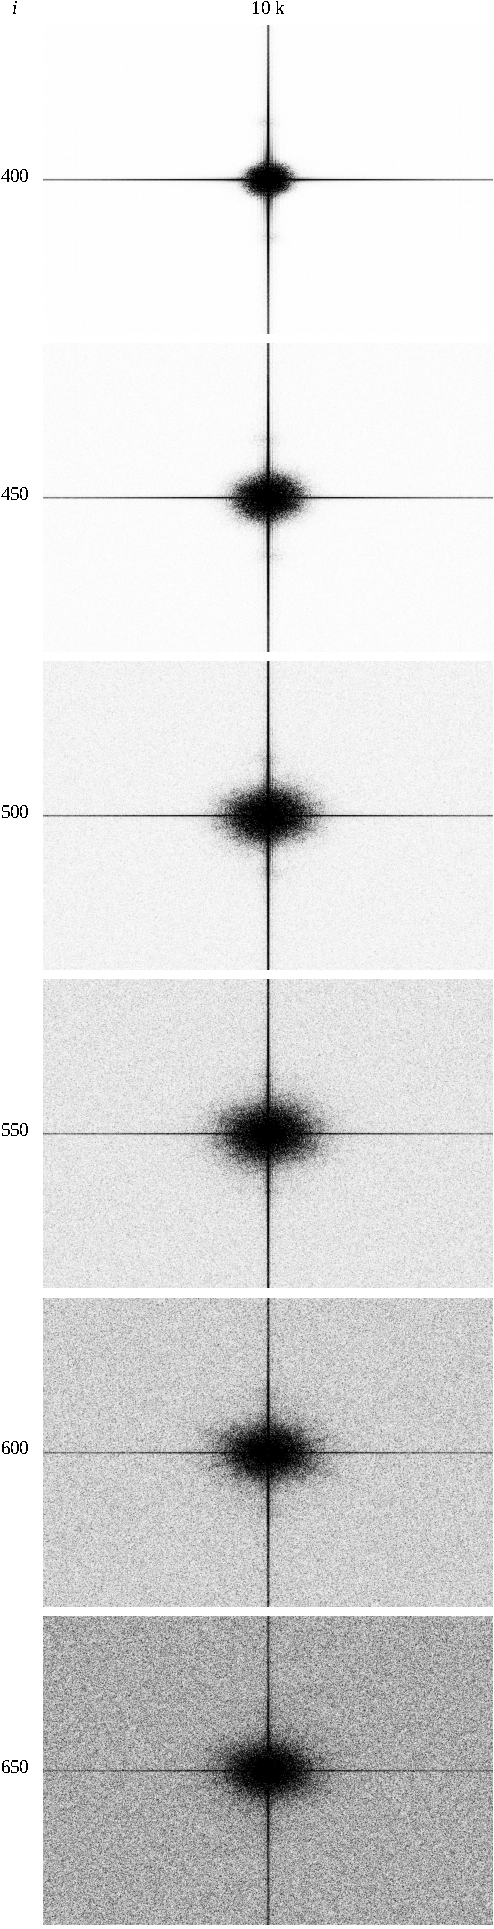
\includegraphics[height=.9\paperheight]{grid10k.pdf}
	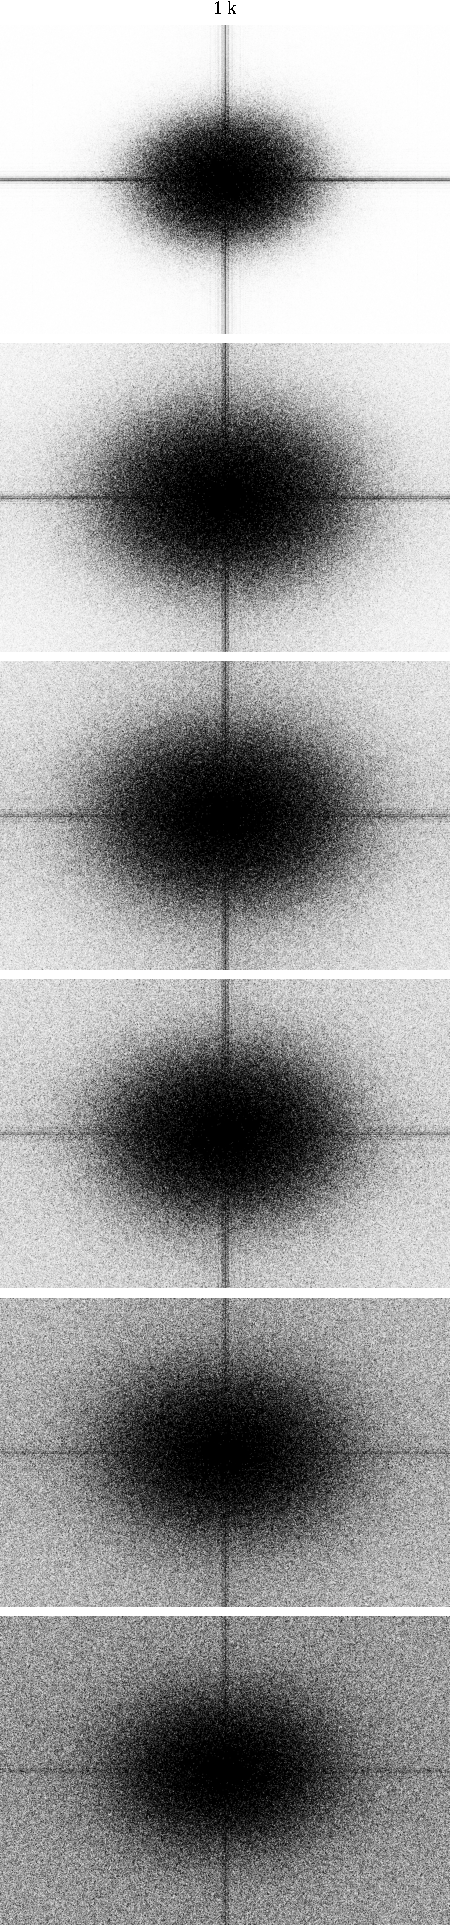
\includegraphics[height=.9\paperheight]{grid1k.pdf}
	\end{minipage}
	\begin{minipage}[c]{.245\linewidth}
	\captionof{figure}[傅立叶]{图 \tup{\ref{fig:photoOriginal}} 的傅立叶频谱}
	\textit{\hphantom{说明}%
		首先看 \SI{10}{k} 倍像,高频成分随$i$增大变得更加复杂,表明图像的细节更加丰富,但同时噪声的成分增大。
	\vspace{-2ex}}\par
	\textit{\hphantom{分析}%
		\SI{1}{k} 倍像的频谱随$i$的变化规律与 \SI{10}{k} 像一致,但由于 \SI{1}{k} 图像对应的表面范围更广,包含更多结构,导致频谱本身的分布范围比 \SI{10}{k} 像来得宽泛,从而高频增强导致的优化效果不如 \SI{10}{k} 倍像那么显著。
	\vspace{1ex}}
	\label{fig:fourier}
	\end{minipage}
	\end{minipage}
\restoregeometry
\FloatBarrier
\clearpage

	本实验对电镜图片像质的评价主要从\textbf{分辨率}这一角度出发;或者,可以直观地认为,对于同一区域的最优化图像,像质的优劣可通过图像所包含\textbf{\CJKunderdot{有效}细节的丰富程度}加以评价。强调细节的有效性,意在将高频噪声排除在外;也就是说,高频噪声对图像的细节也有贡献,但其无益于(甚至有害于)分辨率的提升。
	
	可利用傅立叶变换定量考察图像细节的丰富程度,结果如图 \ref{fig:fourier}. 可以看出,这与直接观察所得的结论一致;也就是说,聚光镜电流越大$i$, 所成像的分辨率越高,但高频噪声的影响也越为显著。
	
	\newparagraph
	下面我们尝试给出这一现象的物理根源。事实上,聚光镜电流$i$越大, 会聚能力越强;这意味着最终到达样品表面的电子“探针”越纤细,电子束斑尺寸越小。根据前述原理部分的讨论,“探针”越纤细,自然导致分辨率越高,从而像质越高。
	
	然而,束斑尺寸还应和系统的采样率(\textit{单位区域内探测器的采样点数目})相匹配。探针过于纤细时,其扫过的点不足以代表整个采样区域,这在图像上体现为随机噪声。权衡以上两大影响因素,可知$i$的选取应当适中;对本实验而言,直观上看,最优像质大致对应$i \approx \numrange{550}{600}$. 
	
	类似的观点也可用于解释其他最优化参数随$i$的变化规律。
	采用光学术语,聚光镜电流增大、会聚能力增强意味着等效的焦距减小。
	而等效的镜筒长度基本固定,为与之匹配,物镜的焦距应相应增大,对应最佳物镜电流减小。
	
	此外,$i$越大,会聚能力越强,出射电子束的发散越显著,导致离轴电子在传播过程中的损失率增大;这导致“探针”的“强度”(束流)变弱,进而导致为二次电子的产量减小,信号减弱;在图像上体现为像的对比度减小,为达到最佳像质,应当相应加大对比度。为了保证图像的表观亮度基本一致,应当相应地减小亮度(\textit{信号的平均强度})。这便解释了表 \ref{tab:bestValues} 中参数的变化规律。
\section{结论}
%%%	首先要给出实验结果,然后再给出由实验结果分析得到的结果和结论.此部分给出的内容要比摘要中的全面,用词要更准确.\par
%%%%%%%%%%%%%%%%%%%%%%%%%%%%%%%
	本实验探究了SEM的基本构造和原理,并进一步考察了聚光镜电流$i$对分辨率的影响,同时探讨了可能的物理机制。实验结果表明,对 \numrange{400}{650} 范围内的$i$值而言,聚光镜电流越大,分辨率越高,但噪声越显著。随后,本文尝试从电子光学的角度对该结果进行了较为合理的解释。对于本仪器(中科科仪KYKY-EM3200型SEM)而言,本文给出建议值$i \approx \numrange{550}{600}$. 
\section{致谢}
%	此部分感谢同组人...和对实验和报告有帮助的人.
%%%%%%%%%%%%%%%%%%%%%%%%%%%%%%
	感谢与我合作的张鹏辉,尤其感谢他在数据统计及仪器启停操作时的出色工作;感谢耐心细致的荀坤老师给我们带来的启发。

\setlength{\bibsep}{2pt}
\linespread{1.2}\selectfont
\bibliographystyle{../BibStyle/gbt-7714-2015-numerical}
\bibliography{../BibStyle/Textbook,bib/Ref}

\clearpage
\appendix
\section*{附\ 实现傅立叶变换的计算代码}
\linespread{1.5}\selectfont
	前述傅立叶变换的数值计算通过 \verb|Mathematica| 实现,核心代码如下:\\[-1.5ex]
	
	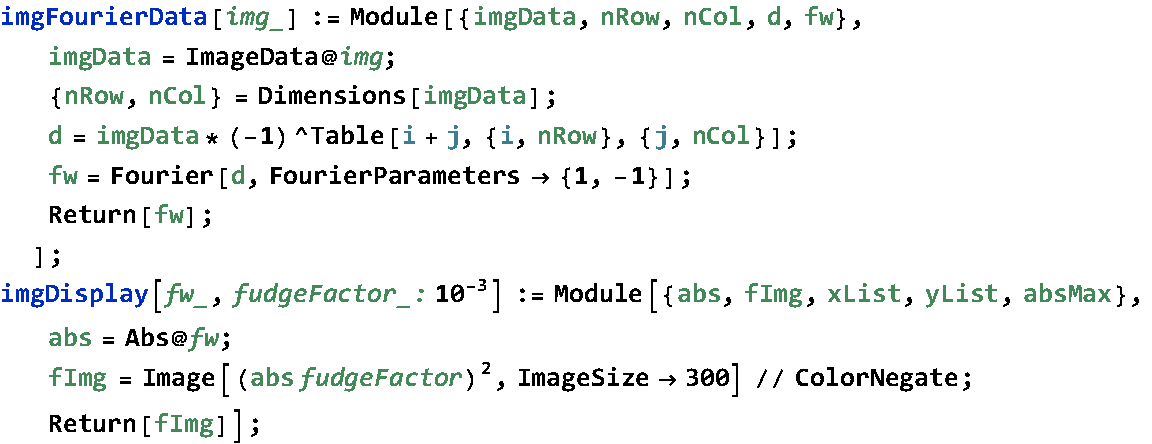
\includegraphics[width=\linewidth]{fourierCode.pdf}
	
	\vspace{.5ex}
	\noindent\textbf{参考:} Mathematica StackExchange, \\[-.8ex] {\hphantom{url:\ \ \ \ }
	\scriptsize\url{https://mathematica.stackexchange.com/questions/29203/calculate-the-2d-fourier-transform-of-an-image}}
\section*{附\ 图像信息量的度量}
	这里我们讨论图像\textit{信息量}的度量方案。这与分辨率有所不同;事实上,分辨率只是表征了图像\textit{局部}的有效信息量。对图像整体而言,图像尺寸越大、分辨率越高,则图像包含的信息量越大。
	
	此外,图像采用的色彩空间(color space)也与其包含的信息量有关;占用的色彩空间越大,信息量越丰富。例如,彩色图像的信息量显然大于黑白图像。
\end{document}
